
\begin{exercise}

 
\begin{minipage}[t]{0.5\textwidth}
Welke snelheid moet een achtbaanwagentje dat op zijn kop boven in een lus aankomt ten minste hebben, willen de passagiers niet naar beneden vallen? Neem aan dat de kromtestraal van de lus $7,0\rm\,m$ bedraagt.
\end{minipage}
\hspace{5mm}
\begin{minipage}[t]{0.45\textwidth}
\raisebox{-2cm}{
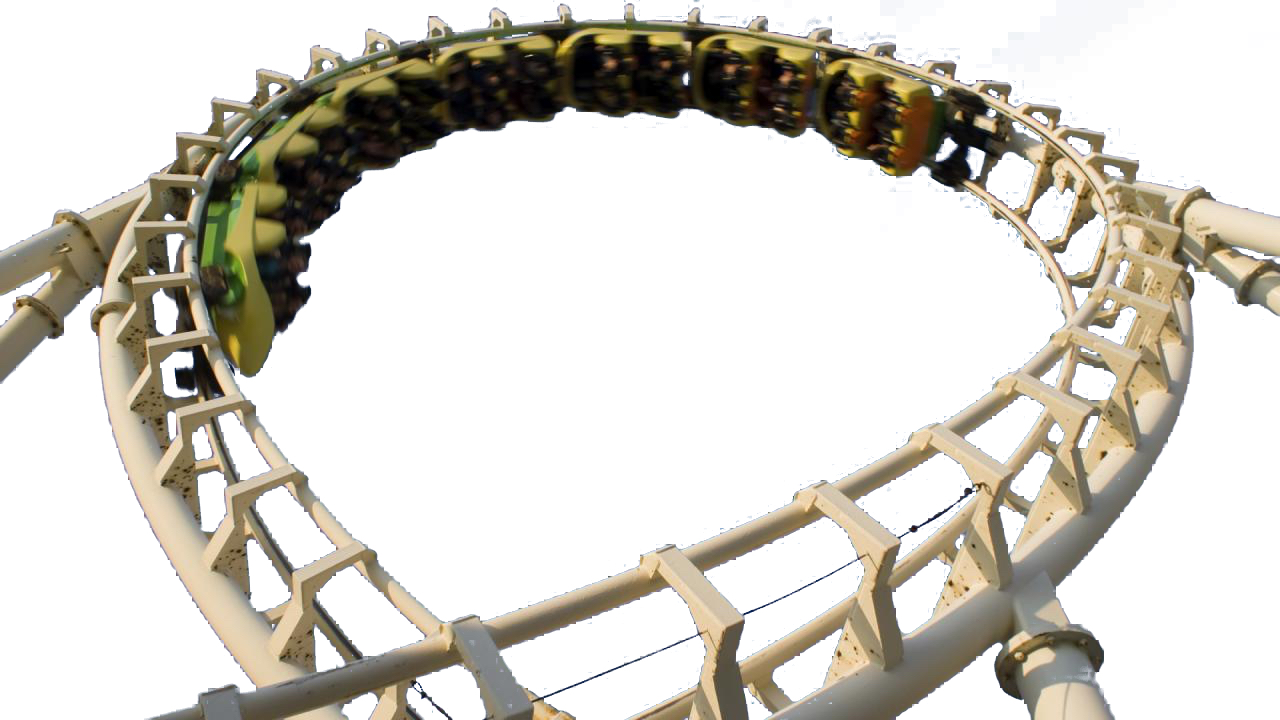
\includegraphics[width=0.9\textwidth]{dyn/exercises/gewonden-ontsporing-achtbaan-vs_res}
}
\end{minipage}
\begin{oplossing}
De snelheid moet groot genoeg zijn zodat de zwaartekracht er niet in slaagt de passagiers sneller uit de bocht te trekken dan noodzakelijk. Hoe trager de passagiers gaan, hoe minder groot de middelpuntzoekende kracht moet zijn om die beweging tot stand te brengen. 
\newline
Bij een snelheid die groot genoeg is, helpt de normaalkracht (door de wagentjes op de passagiers uitgeoefend) de zwaartekracht om een middelpuntzoekende kracht te genereren. De minimale snelheid vinden we dan ook wanneer de normaalkracht wegvalt en enkel de zwaartekracht de middelpuntzoekende kracht levert:
\begin{eqnarray*}
		F=ma\Rightarrow mg=\frac{mv^2}{r}
\end{eqnarray*}
Zodat:
$v_{\rm min}=\sqrt{rg}=8,29\rm\,m/s=29,8\rm\,km/h$.
\end{oplossing}

\end{exercise}
